\chapter{الميكروبيومات والتعايشات}\label{ch:b3:microbiomes}

تحمل في جسدك نحو ثمانية وثلاثين تريليون بكتيريا، أي واحدة
تقريبًا مقابل كل خلية من خلاياك، معظمها في المتر الأخير من
أمعائك، حيث تزن قدر دماغك تقريبًا وتحمل من المورّثات مئة
ضعف ما تحمل أنت. والفأر الذي يُربّى خاليًا منها يحتاج إلى
ثلث إضافي من الغذاء ليحفظ وزنه، وجهازه المناعي ضامر،
وسلوكه شاذ. ونبتة البازلاء تطعم عُشر سكرها بكتيريا في عُقد
على جذورها فتنال النتروجين في المقابل؛ وأربعة أخماس
النباتات البرية كلها \omterm{def:b3:microbiomes:symbiosis}{تقايض} السكر بالفوسفات مع فطور تلتف
حول جذورها، كما تفعل منذ أربعمئة مليون سنة؛ والمرجان حيوان
يزرع طحالب داخل خلاياه ويموت إذا دفئ البحر دفئًا يكفي لأن
يطردها. فالكائنات الحية ليست أفرادًا بل جماعات، ويتناول
هذا الفصل بيولوجيا هذه الشراكات: كيف تُعدّ وتُوصف
بالتسلسل، وما الذي يتبادله الشركاء، وكيف يُتفاوض على
التبادل ويُراقَب، ولماذا ينتهي بعض الشركاء عضيّات.

\section{ألفاظ العيش معًا}

\begin{definition}[التعايش]\label{def:b3:microbiomes:symbiosis}
\index{تعايش}\index{تقايض}\index{معايشة}\index{كائن جامع}\index{ميكروبيوم}\index{انتقال عمودي}
\emph{التعايش} ارتباط دائم وثيق بين كائنات من أنواع
مختلفة؛ وهو \emph{تقايض} إذا ربح الطرفان، و\emph{معايشة}
إذا ربح أحدهما ولم يتأثر الآخر، وتطفّل إذا ربح أحدهما على
حساب الآخر --- وقد ينتقل الزوج نفسه على هذا الخط بتبدل
الظروف. و\emph{المتعايش الداخلي} يعيش داخل خلايا مضيفه؛
و\emph{الشريك الإجباري} لا يقدر على العيش وحده. وتنتقل
المتعايشات \emph{عموديًا}، من الوالد إلى الخلف (فبكتيريا
\emph{Buchnera} في المنّ تمر عبر البيضة)، أو \emph{أفقيًا}،
إذ تُكتسب من جديد في كل جيل من البيئة أو من مضائف أخرى
(بكتيريا \emph{Vibrio} في الحبّار، وبكتيريا أمعاء الإنسان).
و\emph{الميكروبيوم} هو جماعة الميكروبات كلها في موئل ---
أمعاء، أو سطح ورقة، أو غرام من التربة --- و\emph{الكائن
الجامع} هو المضيف مع ميكروبيومه، منظورًا إليهما وحدةً
يراها الانتخاب الطبيعي.
\end{definition}

\begin{example}[ثلاثة شركاء إجباريين]\label{ex:b3:microbiomes:obligate}
عاشت \emph{Buchnera} في خلايا مضيفها المنّ مئتي مليون سنة،
وهي تصنع الأحماض الأمينية الأساسية التي يفتقر إليها عصير
اللحاء، وقد قلّصت جينومها إلى \qty{640}{kb} --- سُبع جينوم
أقاربها الحرة --- فأضاعت كل مورّثة صار المضيف يوفّر
منتجها. وبكتيريا \emph{Wolbachia}، الموجودة في ثلثي أنواع
الحشرات، لا تنتقل إلا عبر البيوض، فتطورت لتؤثر الإناث:
تقتل الأجنة الذكور، أو تؤنثها، أو تجعل بيوض الإناث غير
المصابة تموت إذا لقّحتها ذكور مصابة (\emph{عدم التوافق
السيتوبلازمي})، وهو ما ينشرها في الجمهرة؛ والبعوض الحامل
لها ينقل حمى الضنك نقلًا رديئًا، وقد خفض إطلاقه الضنك في
عدة مدن. وأما أميبة \emph{Paulinella} فقد ضمّت إليها
زُراقم قبل نحو مئة مليون سنة، وهي اليوم ليست بكتيريا تمامًا
ولا بلاستيدة خضراء تمامًا --- أي أصل ثانٍ مستقل للعضيات
الضوئية، أُمسك في منتصف الطريق.
\end{example}

\section{عدّ جماعة}

\begin{method}[توصيف ميكروبيوم بالتسلسل]\label{met:b3:microbiomes:16s}
\index{تسلسل 16S rRNA}\index{ميتاجينوميات}\index{وحدة تصنيفية إجرائية}
معظم الميكروبات لا يمكن استنباتها؛ وإنما تُعدّ بحمضها
النووي. (1) استخلص DNA من العينة --- براز، أو تربة، أو ماء
بحر مُرشَّح على غشاء. (2) ثم إما أن تضخّم مورّثة RNA
الريبوزومي للوحيدة الصغرى (\emph{16S}) ببادئات تطابق
مناطقها الكونية، وتُسلسل المناطق المتغيرة بينها --- وهو
مسح \emph{المُضخَّمات}، رخيص، يعرّف البكتيريا إلى حدود
الجنس ويعدّها بعدد القراءات؛ وإما أن تُسلسل DNA كله ---
\emph{ميتاجينوميات البندقية}، وهي تستعيد المورّثات
والجينومات الكاملة فتخبر بما تقدر عليه الجماعة، لا بمن
فيها فحسب. (3) اجمع القراءات في متغيرات تسلسلية أو
\emph{\omterm{met:b3:microbiomes:16s}{وحدات تصنيفية إجرائية}} (OTU، وهي اصطلاحًا عند تطابق
\qty{97}{\%} لأجل ``نوع'')، وأسندها بالمقارنة مع قواعد
البيانات (\cref{ch:b3:bioinformatics})، وجدول الأعداد في كل
عينة. (4) احسب التنوع داخل العينة وقارن التركيب بين
العينات. والأعداد نسبية --- إذ تجمع قراءات العينة إلى مجموع
ثابت --- وتتحيزها طرق الاستخلاص والبادئات وعدد النسخ،
فالفروق بين عينات عولجت المعالجة نفسها جديرة بالثقة حيث لا
تكون الأعداد المطلقة كذلك.
\end{method}

\begin{definition}[التنوع]\label{def:b3:microbiomes:diversity}
\index{غنى نوعي}\index{دليل شانون}\index{دليل سيمبسون}\index{ترقيق}
لجماعة فيها $S$ نوعًا وفراتها النسبية $p_{1},\dots,
p_{S}$ ($\sum p_{i} = 1$): \emph{الغنى} هو $S$؛ و\emph{دليل
شانون} $H = -\sum_{i} p_{i}\ln p_{i}$ يقيس الارتياب في نوع
فرد يُسحب عشوائيًا، و$e^{H}$ هو عدد الأنواع المتساوية
الوفرة الذي يعطي الارتياب نفسه (العدد الفعال للأنواع)؛
و\emph{دليل سيمبسون} $D = \sum_{i} p_{i}^{2}$ هو احتمال أن
يكون فردان يُسحبان عشوائيًا من النوع نفسه، و$1/D$ عدد فعال
آخر، مرجَّح نحو الأنواع الشائعة. ويتوقف الغنى على عدد
الأفراد الذين نُظر فيهم: و\emph{منحنى الترقيق} يرسم
الأنواع الموجودة في مقابل عدد الأفراد المعاينين، ويستوي حين
تكون معظم الأنواع قد رُئيت.
\end{definition}

\begin{theorem}[الترقيق]\label{thm:b3:microbiomes:rarefaction}
\index{ترقيق!صيغة}\index{تغطية غود}
عينة فيها $N$ فردًا من $S$ نوعًا، منها $N_{i}$ من النوع
$i$. فالعدد المتوقع للأنواع في عينة جزئية عشوائية من $n$
فردًا، مسحوبة بلا إرجاع، هو
\[
E[S_{n}] = \sum_{i=1}^{S}\left[1 - \frac{\binom{N - N_{i}}{n}}
{\binom{N}{n}}\right],
\]
وهو يرتفع مع $n$ ويساوي $S$ عند $n = N$. وتُقارن عينتان
مختلفتا الحجم بترقيقهما إلى $n$ واحد. وأما نسبة أفراد
الجماعة التي تنتمي إلى أنواع لم تُرَ بعد فتُقدَّر من
\emph{\omterm{thm:b3:microbiomes:rarefaction}{تغطية غود}}: نحو $f_{1}/N$، حيث $f_{1}$ عدد الأنواع
التي رُئيت مرة واحدة بالضبط (المفردات).
\end{theorem}
\begin{proof}
يغيب النوع $i$ عن العينة الجزئية بالضبط حين تُسحب أفرادها
$n$ كلها من الأفراد $N - N_{i}$ الآخرين، وهو ما يقع في
$\binom{N - N_{i}}{n}$ من العينات الجزئية $\binom{N}{n}$
المتساوية الاحتمال؛ فالنوع $i$ حاضر باحتمال $1 - \binom{N-N_{i}}{n}/
\binom{N}{n}$، والعدد المتوقع للأنواع الحاضرة هو مجموع هذه
الاحتمالات (توقع مجموع مُشعِرات). وكل حد يزداد مع $n$، وعند
$n = N$ يكون كل مُعامل ثنائي في البسط صفرًا. وأما تقدير
غود: فالفرد الذي يُسحب تاليًا ينتمي إلى نوع لم يُرَ
باحتمال يقارب احتمال أن يكون فرد يُختار عشوائيًا من العينة
وحيد نوعه، أي $f_{1}/N$ (غود، 1953)؛ وتبريره مُسلَّم به
هنا.
\end{proof}

\begin{example}[أمعاء اثنين]\label{ex:b3:microbiomes:two-guts}
عينة من $1000$ قراءة من شخص تعطي $150$ نوعًا، مع
$H = 3.5$ و$40$ نوعًا مفردًا؛ وعينة من $5000$ قراءة من شخص
آخر تعطي $260$ نوعًا. وليست الثانية أكثر تنوعًا بالضرورة:
فقد عوينت خمس مرات أعمق، وترقيقها إلى $1000$ قراءة قد يعطي
$150$ أيضًا. وتغطية العينة الأولى $1 - 40/1000 =
\qty{96}{\%}$: أي أن أربعة في المئة من بكتيريا تلك الأمعاء
تنتمي إلى أنواع لم ترها العينة قط، وستجدها عينة أعمق.
والأعداد الفعالة، $e^{3.5} \approx 33$ نوعًا من حيث
التساوي في مقابل غنى قدره $150$، تقول إن أنواعًا قليلة
تهيمن --- وهكذا تبدو كل أمعاء.
\end{example}

\begin{omfigure}
\begin{tikzpicture}
\begin{axis}[
  width=0.68\linewidth, height=5.6cm,
  axis x line=bottom, axis y line=left,
  xmin=0, xmax=5000, ymin=0, ymax=300,
  xlabel={القراءات المعاينة، $n$}, ylabel={الأنواع المرصودة},
  xlabel style={font=\small, at={(axis description cs:0.5,-0.12)}, anchor=north}, ylabel style={font=\small},
  tick label style={font=\small}, xtick={0,1000,2000,3000,4000,5000}, ytick={0,100,150,200,260},
  clip=false,
]
\addplot[very thick, omDef, domain=0:5000, samples=60] {260*(1-exp(-x/1500))};
\addplot[very thick, omThm, domain=0:1000, samples=30] {150*(1-exp(-x/300))*1.0};
\addplot[very thick, omThm, dashed, domain=1000:5000, samples=30] {150*(1-exp(-x/300))*1.0 + 8*(1-exp(-(x-1000)/2000))};
\draw[dashed, gray] (axis cs:1000,0) -- (axis cs:1000,300);
\node[font=\scriptsize, omDef, anchor=north west] at (axis cs:1200,292) {الأمعاء الثانية: $260$ نوعًا عند $5000$ قراءة};
\node[font=\scriptsize, omThm, anchor=north east] at (axis cs:4900,140) {الأمعاء الأولى: $150$ عند $1000$، قرب استوائها};
\node[font=\scriptsize, gray, anchor=south west] at (axis cs:1050,10) {رقّق هنا للمقارنة};
\end{axis}
\end{tikzpicture}

{\small منحنيات \omterm{def:b3:microbiomes:diversity}{الترقيق}. ترتفع الأنواع الموجودة مع عدد
القراءات المعاينة وتستوي حين تُستنفد الجماعة؛ وتُقارن
عينتان عند العمق نفسه. وهنا لا تزال الأمعاء الثانية صاعدة
عند $5000$ قراءة، فغناها الحقيقي أعلى بعد.}
\end{omfigure}

\section{الميكروبيوم البشري}

\begin{definition}[جماعة الأمعاء]\label{def:b3:microbiomes:gut}
\index{ميكروبيوم الأمعاء}\index{حمض دهني قصير السلسلة}\index{مقاومة الاستعمار}\index{خلل التوازن الجرثومي}
تحوي أمعاء الإنسان نحو $4\times 10^{13}$ بكتيريا، جلّها في
القولون عند $10^{11}$ لكل غرام من المحتويات، في مقابل
$10^{3}$ لكل غرام في المعدة الحمضية و$10^{4}$--$10^{7}$ على
امتداد المعي الدقيق، حيث الجريان سريع والصفراء معادية.
وفيها من خمسمئة إلى ألف نوع في الشخص الواحد، معظمها من
شعبتين، الباكتيرويديتات والفيرميكوتات، وكلها تقريبًا
لاهوائية؛ ومجموعة كل شخص متميزة وثابتة سنين، تتثبت في
معظمها في السنوات الثلاث الأولى من العمر من الأم ومن أهل
البيت. وما تفعله: تخمّر الألياف التي تعجز إنزيمات الإنسان
عن هضمها فتحيلها \emph{أحماضًا دهنية قصيرة السلسلة} ---
الخلات، والبروبيونات، والبوتيرات --- تغذي خلايا القولون
نفسها وتوفر حتى عُشر سعرات المضيف؛ وتصنع فيتامين~K وبعض
فيتامينات B؛ وتحوّل الأحماض الصفراوية والأدوية؛ وتشغل كل
كوّة حتى لا يجد غازٍ موطئ قدم (\emph{مقاومة الاستعمار})؛
وتدرّب الجهاز المناعي، إذ تنمو خلاياه التائية النظيمية
وخلاياه المفرزة للغلوبولين IgA استجابةً لها
(\cref{ch:b3:adaptive-immunity}). والجماعة التي تزيح عن هذه
الحالة --- أنواع أقل، ومخمّرات أقل، وهوائيات اختيارية أكثر
--- هي \emph{خلل توازن جرثومي}، يُرى في داء الأمعاء
الالتهابي، وبعد الصادات، وفي البدانة، وإن كان أيهما السبب
وأيهما النتيجة غير واضح عادةً.
\end{definition}

\begin{proof}[شواهد]
الفئران التي تُربّى خالية من الجراثيم في عوازل معقمة
(غوردون وزملاؤه، العقد الأول من هذا القرن) جدرها المعوية
رقيقة، وأعضاؤها اللمفية صغيرة، ومستويات أضدادها منخفضة،
وتحتاج إلى \qty{30}{\%} سعرات أكثر لتحفظ وزنها؛ فإذا
استُعمرت بجراثيم فأر سويّ اكتسبت شحمًا في أسبوعين. وإذا
أُعطيت جراثيم فأر بدين بدل فأر نحيل، اكتسبت الفئران
الخالية من الجراثيم شحمًا أكثر على الطعام نفسه (تورنبو،
2006): فالجماعة نفسها تؤثر في حصاد الطاقة. وفي البشر، شُفي
التهاب القولون المعاود بجرثوم \emph{Clostridioides
difficile} --- وهو خلل توازن أزالت فيه الصادات منافسي
متبوّغ ينتج ذيفانًا --- في \qty{94}{\%} من المرضى بحقن براز
متبرع سليم، في مقابل \qty{31}{\%} بالصاد المعياري (فان نود،
2013)، وهي أول تجربة معشّاة كان فيها الدواء جماعةً لا
جزيئًا.
\end{proof}

\begin{omfigure}
\begin{tikzpicture}
\begin{axis}[
  width=0.68\linewidth, height=5.4cm,
  ybar, bar width=18pt,
  axis x line=bottom, axis y line=left,
  ymode=log, ymin=1, ymax=1e13,
  symbolic x coords={stomach, duodenum, jejunum, ileum, colon},
  xticklabels={المعدة, العفج, الصائم, اللفائفي, القولون},
  xtick=data, ytick={1e1,1e3,1e5,1e7,1e9,1e11},
  ylabel={بكتيريا لكل غرام من المحتويات},
  ylabel style={font=\small}, tick label style={font=\small},
  clip=false,
]
\addplot[fill=omDef!40, draw=omDef] coordinates {(stomach,1e3) (duodenum,1e4) (jejunum,1e5) (ileum,1e7) (colon,1e11)};
\node[font=\scriptsize, anchor=west, xshift=10pt] at (axis cs:stomach,3e3) {حمضية، pH 2};
\node[font=\scriptsize, anchor=south] at (axis cs:jejunum,1.5e5) {صفراء، جريان سريع};
\node[font=\scriptsize, anchor=south, align=center] at (axis cs:colon,1.5e11) {بطيء، لاهوائي:\\المخمِّر};
\end{axis}
\end{tikzpicture}

{\small كثافة البكتيريا على امتداد أمعاء الإنسان، بمقياس
لوغاريتمي: ارتفاع بمئة مليون ضعف من المعدة الحمضية إلى
القولون، حيث تعيش ميكروبات الجسم كلها تقريبًا.}
\end{omfigure}

\begin{omfigure}
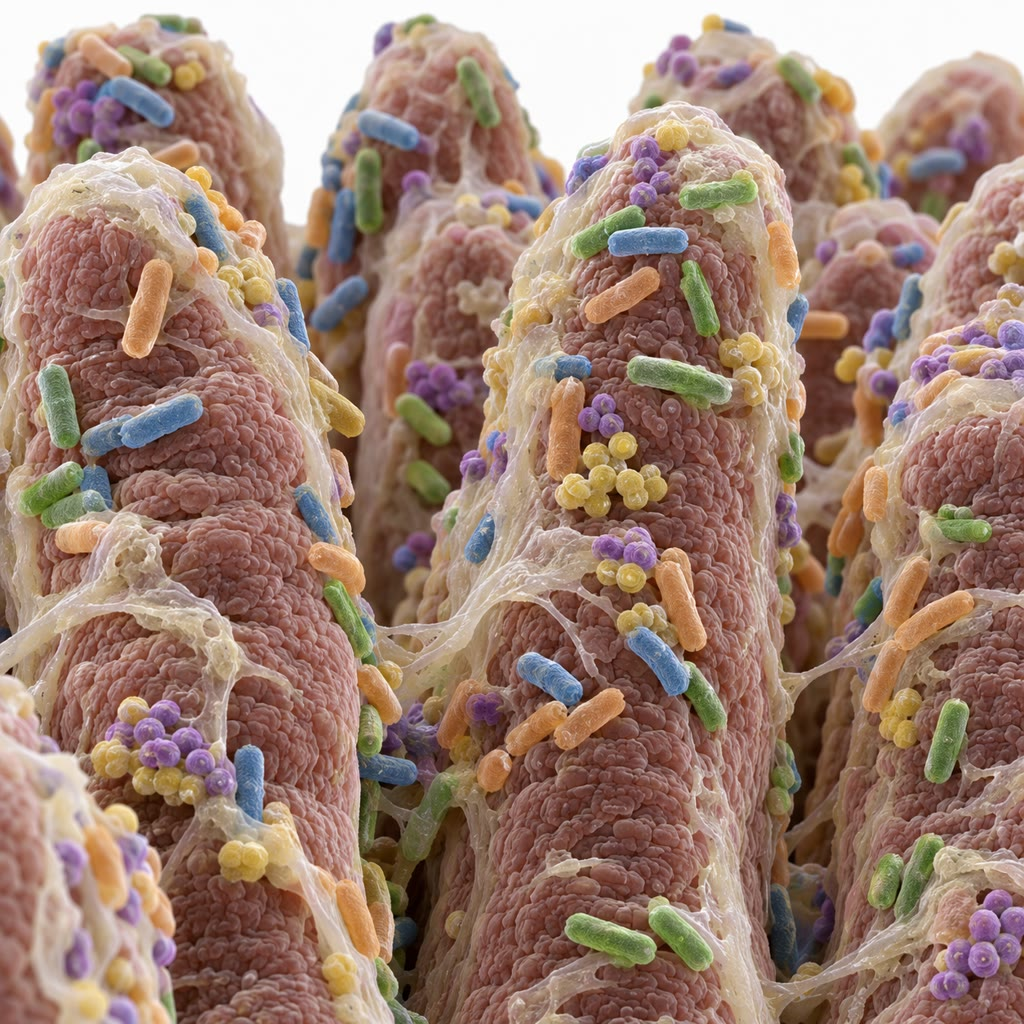
\includegraphics[width=0.40\linewidth]{images/book5/ai/b5-14-gut-microbiota.jpg}

{\small سطح بطانة المعي في المجهر الإلكتروني الماسح،
وبكتيريا من أنواع عدة مستقرة في المخاط بين الزغابات.}
\end{omfigure}

\section{النباتات وشركاؤها}

\begin{definition}[تعايش البقولية والريزوبيوم]\label{def:b3:microbiomes:nodule}
\index{ريزوبيا}\index{عقدة جذرية}\index{عامل Nod}\index{ليغهيموغلوبين}\index{نتروجيناز}
تؤوي البقوليات بكتيريا مثبتة للنتروجين (\emph{الريزوبيا})
في \emph{عُقد جذرية}، وهي أعضاء تُبنى لهذا الغرض بعد حوار
جزيئي. فالجذر يفرز الفلافونيدات؛ ويجيب ريزوبيوم من النوع
المطابق بإفراز \emph{عوامل Nod} --- وهي سكريات شحمية
كيتينية قليلة تحدد زخارفُها الشريك؛ ويربطها مستقبل كيناز
على شعرة الجذر فيطلق تذبذبات الكالسيوم في النواة، والتفاف
شعرة الجذر حول البكتيريا، و\emph{خيط إصابة} ينمو إلى
الداخل عبر الخلايا بينما تبدأ القشرة تحته بالانقسام لتصير
عقدة. وتُطلق البكتيريا في خلايا العقدة داخل أغشية فتتمايز
إلى \emph{بكتيرويدات} تعبّر عن \emph{النتروجيناز}، وهو
الإنزيم الذي يرد N$_{2}$ إلى نشادر بكلفة ستة عشر ATP
للجزيء الواحد. ويهدم الأكسجين النتروجيناز، مع أن
البكتيرويدات تتنفس بشدة؛ وتحل العقدة التناقض بحاجز انتشار،
وبصبغة \emph{الليغهيموغلوبين}، وهي هيموغلوبين نباتي يربط
الأكسجين ربطًا محكمًا وينقله إلى البكتيرويدات عند تركيز حر
منخفض --- وهي ما يجعل العقدة المقطوعة وردية. ويدفع النبات
ستة إلى عشرة في المئة من نواتج تركيبه الضوئي وينال معظم
نتروجينه؛ ويقارب النتروجين المثبَّت في محاصيل البقوليات في
العالم ما تثبته صناعة الأسمدة.
\end{definition}

\begin{omfigure}
\begin{tikzpicture}[every node/.style={font=\scriptsize}, >=stealth]
  % stage 1: root hair and bacteria, flavonoid / Nod factor exchange
  \begin{scope}
    \draw[thick, omMeth!60!black, fill=omMeth!15] (0,0) rectangle (1.2,3.0);
    \draw[thick, omMeth!60!black, fill=omMeth!15] (1.2,1.6) .. controls (2.4,1.7) and (2.6,2.6) .. (2.9,2.4) .. controls (2.5,2.3) and (2.3,1.4) .. (1.2,1.2) -- cycle;
    \foreach \p in {(3.1,2.7),(3.4,2.3),(3.3,1.9)} \fill[omProp] \p ellipse (0.14 and 0.07);
    \draw[->, omMeth!60!black, thick] (2.6,1.5) -- (3.2,1.4); \node[below, omMeth!60!black] at (3.0,1.35) {الفلافونيدات};
    \draw[<-, omProp, thick] (2.5,2.85) -- (3.0,3.0); \node[above, omProp] at (2.4,2.95) {عوامل Nod};
    \node[below, align=center] at (1.6,-0.2) {1. حوار: شعرة الجذر\\والريزوبيا};
  \end{scope}
  % stage 2: curled hair, infection thread
  \begin{scope}[xshift=4.6cm]
    \draw[thick, omMeth!60!black, fill=omMeth!15] (0,0) rectangle (1.2,3.0);
    \draw[thick, omMeth!60!black, fill=omMeth!15] (1.2,1.6) .. controls (2.3,1.8) and (2.8,2.6) .. (2.2,2.8) .. controls (1.9,2.9) and (1.8,2.5) .. (2.0,2.4) .. controls (2.3,2.2) and (1.9,1.3) .. (1.2,1.2) -- cycle;
    \draw[omProp, very thick] (2.05,2.55) .. controls (1.8,2.1) and (1.4,1.7) .. (0.4,1.3);
    \foreach \p in {(1.85,2.3),(1.5,1.9),(1.1,1.6),(0.7,1.4)} \fill[omProp] \p ellipse (0.1 and 0.05);
    \node[right, omProp, font=\tiny] at (2.3,1.0) {خيط الإصابة};
    \foreach \p in {(0.3,0.5),(0.6,0.7),(0.9,0.5)} \draw[omMeth!60!black] \p circle (0.12);
    \node[below, align=center] at (1.6,-0.2) {2. تلتف الشعرة؛ وينمو الخيط داخلًا؛\\وتنقسم خلايا القشرة};
  \end{scope}
  % stage 3: nodule
  \begin{scope}[xshift=9.0cm]
    \draw[thick, omMeth!60!black, fill=omMeth!15] (0,0) rectangle (1.2,3.0);
    \draw[thick, omThm!60!black, fill=omThm!25] (1.2,1.5) ellipse (1.3 and 1.0);
    \foreach \p in {(1.0,1.5),(1.5,1.8),(1.6,1.2),(1.1,1.9),(1.2,1.1),(2.0,1.5)} \fill[omProp] \p circle (0.1);
    \node[right, align=left] at (2.6,2.0) {عقدة: بكتيرويدات\\فيها نتروجيناز};
    \node[right, align=left, omThm!60!black] at (2.6,1.1) {وردية: الليغهيموغلوبين\\يبقي O$_2$ منخفضًا};
    \draw[->, thick] (0.6,2.4) -- (1.0,2.0) node[pos=0, above] {سكر};
    \draw[<-, thick] (0.6,0.6) -- (1.0,1.0) node[pos=0, below] {NH$_3$};
    \node[below, align=center] at (1.6,-0.2) {3. تثبّت البكتيرويدات N$_2$؛\\سكر مقابل نشادر};
  \end{scope}
\end{tikzpicture}

{\small صنع عقدة. تعرّف الفلافونيداتُ الآتية من الجذر
وعواملُ Nod الآتية من الريزوبيوم كلًّا من الشريكين؛ ثم
تلتف شعرة الجذر، ويحمل خيط الإصابة البكتيريا إلى الداخل،
وتبني القشرة عقدةً تثبّت فيها البكتيرويدات، التي يبقيها
\omterm{def:b3:microbiomes:nodule}{الليغهيموغلوبين} عند أكسجين منخفض، النتروجين مقابل السكر.}
\end{omfigure}

\begin{definition}[الميكوريزات]\label{def:b3:microbiomes:mycorrhiza}
\index{ميكوريزا}\index{ميكوريزا شجيرية}\index{سبيل التعايش المشترك}
\emph{الميكوريزات} ارتباطات بين الجذور والفطور، توجد في
نحو \qty{80}{\%} من أنواع النبات وفي أقدم أحافير النبات
البري. ففي \emph{الميكوريزات الشجيرية} يدخل الفطر (من
الغلوميروميسيتات) خلايا الجذر ويتفرع إلى شُجيرة شبيهة
بالشجرة يعبرها الفوسفات والنتروجين والماء إلى النبات،
والسكريات والدهون إلى الفطر؛ وتمدّ الخيوط الفطرية سطح
الامتصاص في الجذر مئة ضعف وتبلغ فوسفاتًا لا يبلغه الجذر.
وفي \emph{الميكوريزات الخارجية}، وهي ميكوريزات أشجار
الغابة، يغلّف الفطر الجذر وينمو بين الخلايا. ومورّثات
النبات التي تأذن للفطر هي نفسها \emph{سبيل \omterm{def:b3:microbiomes:symbiosis}{التعايش}
المشترك} --- مستقبل، وتذبذب كالسيوم، وعوامل استنساخ ---
الذي تعيد البقوليات استعماله \omterm{def:b3:microbiomes:nodule}{للريزوبيا}: فالعقدة ابتكار
متأخر بُني على شراكة فطرية تكبرها بأربعمئة مليون سنة.
\end{definition}

\begin{proposition}[المقايضة وضبطها]\label{prop:b3:microbiomes:sanctions}
\index{اختيار الشريك}\index{عقوبات}\index{غشّاش}
\omterm{def:b3:microbiomes:symbiosis}{التقايض} مبادلة، وكل شريك منتخَب ليعطي أقل ويأخذ أكثر؛
وإنما يدوم لأن الشريك الآخر يقدر على الرد. فالبقوليات تحدّ
من الأكسجين في العقد التي لا تثبّت ريزوبياها نتروجينًا
فتنصّف تكاثرها (كيرز، 2003): وتلك \emph{العقوبات}.
والنباتات في الشبكات الميكوريزية تخصص كربونًا أكثر للشركاء
الفطريين الذين يسلّمون فوسفاتًا أكثر، وتخصص الفطور
فوسفاتًا أكثر للجذور التي تدفع كربونًا أكثر --- سوق يكافئ
فيها الطرفان المقايض الأفضل (كيرز، 2011). والحبّار يطرد
بكتيريا عضوه الضيائي التي لا تضيء؛ وجهاز الإنسان المناعي
يتحمل المعايشات التي تبقى في اللمعة ويهاجم التي تعبر
الجدار. وحيث لا يقدر المضيف على الاختيار ولا على المعاقبة
--- كمتعايش داخلي يُورَّث عبر البيضة --- يأتي توافق
المصالح من المصير المشترك: فالمتعايش المنتقل عموديًا لا
يتكاثر إلا حين يتكاثر مضيفه، والانتخاب عليه يحابي تكاثر
المضيف. فطريقة الانتقال تنبئ إذن بطبيعة الشراكة: \omterm{def:b3:microbiomes:symbiosis}{الانتقال
العمودي} نحو \omterm{def:b3:microbiomes:symbiosis}{التقايض} والتبعية، والانتقال الأفقي نحو
الاستغلال الذي يكبحه الضبط.
\end{proposition}
\admitted

\begin{omfigure}
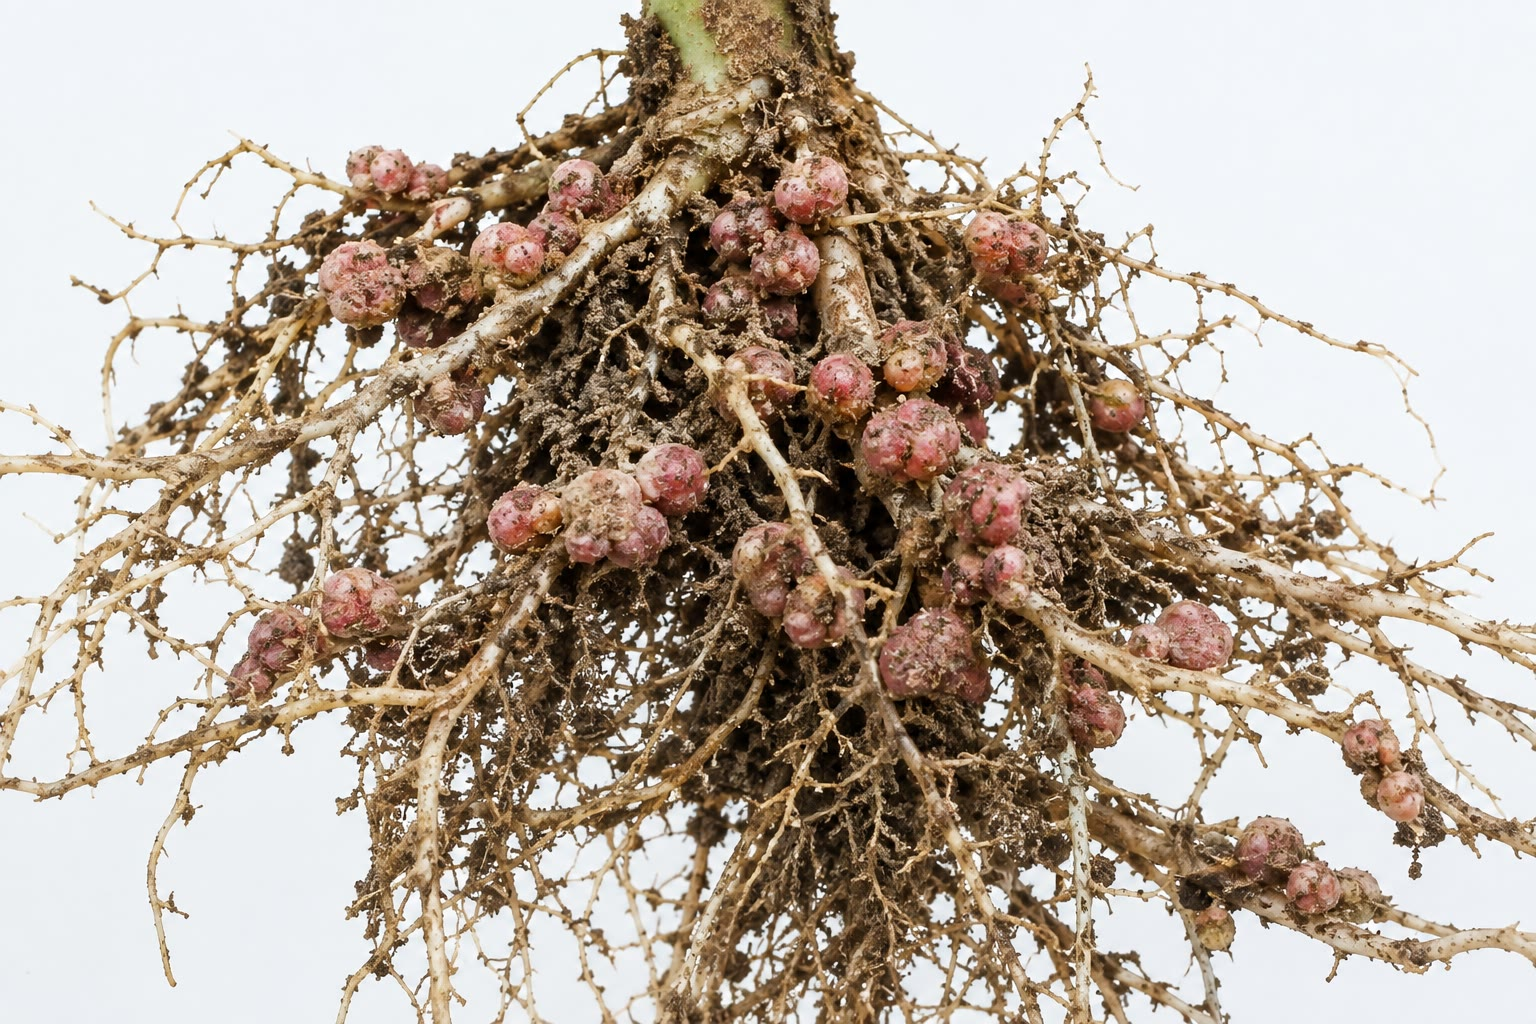
\includegraphics[width=0.46\linewidth]{images/book5/ai/b5-14-root-nodules.jpg}\hspace{0.04\linewidth}
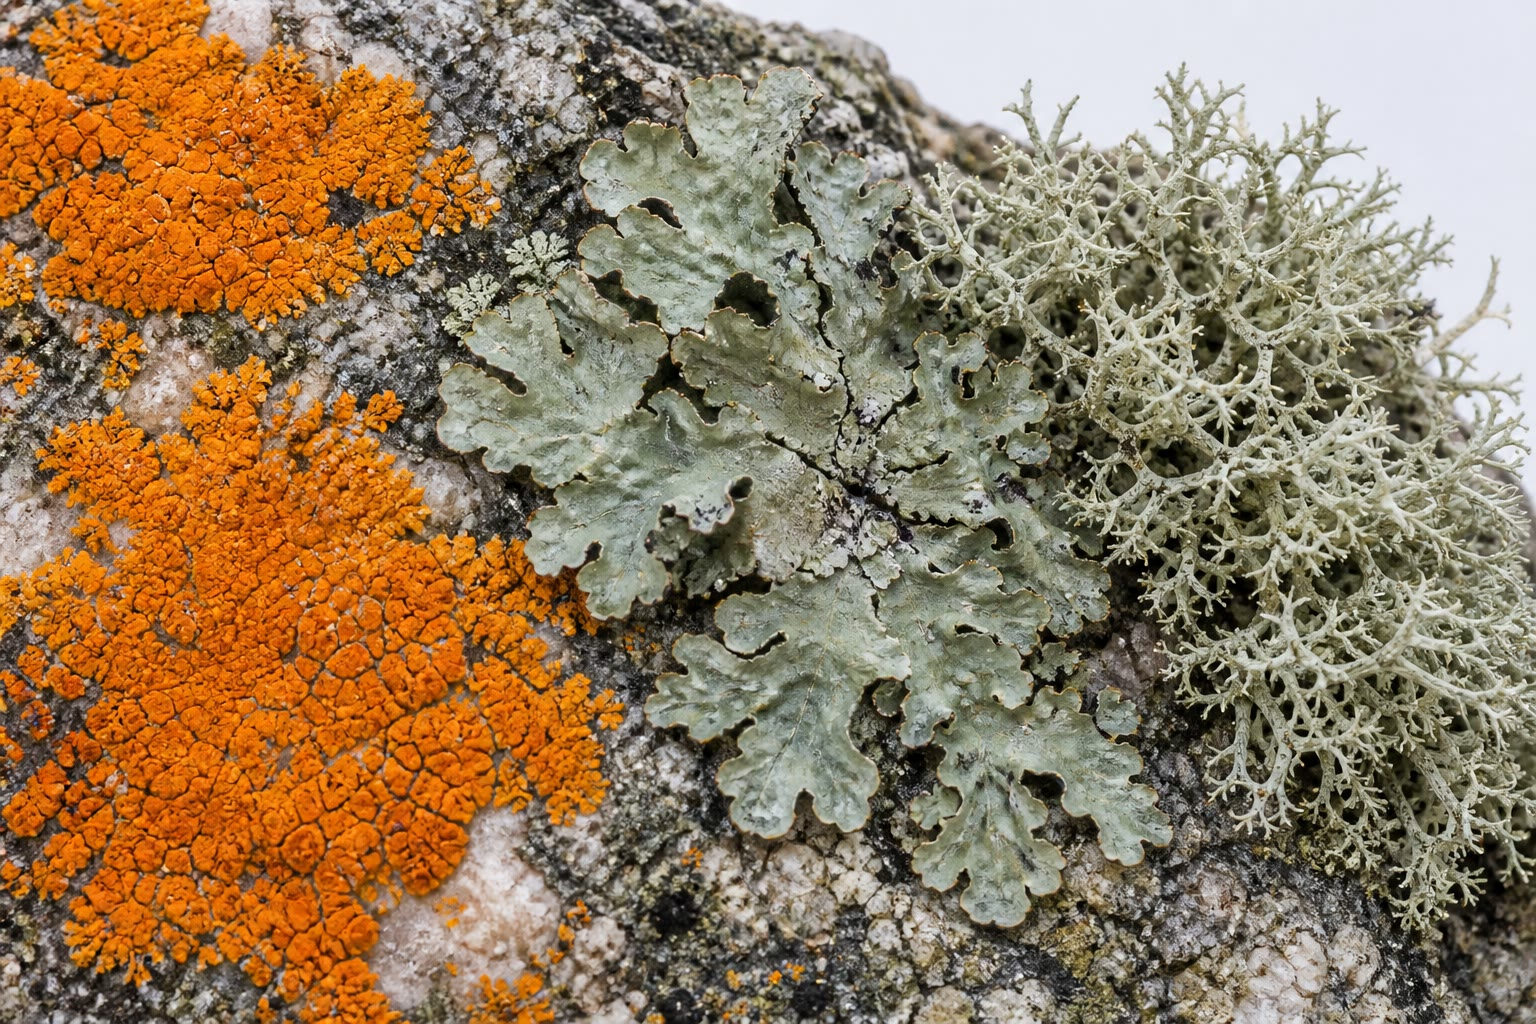
\includegraphics[width=0.46\linewidth]{images/book5/ai/b5-14-lichen.jpg}

{\small يسارًا: جذور بقولية معقّدة، كل عقدة وردية فيها
مصنع نتروجين من بكتيرويدات تُطعَم سكرًا. ويمينًا: أشنات
على صخر --- كل واحدة فطر يؤوي طحلبًا ضوئيًا أو زُراقم،
يستعمران معًا سطحًا لا يقوى عليه أحدهما وحده.}
\end{omfigure}

\section{شراكات في البحر وغيره}

\begin{definition}[المرجان والطحلب]\label{def:b3:microbiomes:coral}
\index{تعايش المرجان}\index{زوزانثيلات}\index{ابيضاض المرجان}
تؤوي مرجانيات بناء الشعاب طحالب سوطية ثنائية
(\emph{Symbiodiniaceae}، أي \emph{الزوزانثيلات}) داخل خلايا
بطانة معيها، مليونًا أو أكثر في السنتيمتر المربع. وتقوم
الطحالب بالتركيب الضوئي في نسيج الحيوان، مستعملة ما يطرحه
من CO$_{2}$ ونشادر وفوسفات، وتعيد إليه حتى \qty{90}{\%} من
كربونها المثبَّت غليسرولًا وسكريات وأحماضًا أمينية، تغذي
المرجان والتكلس الذي يبني الشعبة؛ ويتحكم المرجان في
المقابل بإمداد الطحالب بالنتروجين ومن ثم بنموها. وتعمل
الشراكة ضمن نافذة حرارية ضيقة: فإذا بقي الماء درجة أو
درجتين فوق العظمى الصيفية بضعة أسابيع، تضرر التركيب الضوئي
في الطحالب، فأطلقت أكسجينًا فعالًا في خلايا المضيف، فطردها
المرجان --- وذلك \emph{الابيضاض}، إذ يظهر الهيكل الأبيض من
وراء الحيوان الشفيف. والمرجان المبيضّ يجوع؛ فيتعافى إن برد
الماء في غضون أسابيع، ويموت إن لم يبرد. وقد ارتفع تواتر
الابيضاض خمسة أضعاف منذ 1980، وهو الآلية التي يزيل بها
الاحترار الشعاب.
\end{definition}

\begin{example}[تعايشات تصنع موائل]\label{ex:b3:microbiomes:habitats}
\emph{الأشنة} فطر يؤوي طحلبًا أخضر أو زُراقم، يوفر الفطر
البنية وحفظ الماء والمعادن المذابة من الصخر، ويوفر الرفيق
الضوئي السكر (والنتروجين إن كان زُراقم)؛ وتغطي الأشنات نحو
\qty{8}{\%} من سطح اليابسة، وتستعمر الصخر العاري، وتبدأ
تحويله تربةً. والدودة الأنبوبية \emph{Riftia} في الفوّهات
العميقة لا فم لها ولا معي في طور البلوغ؛ وإنما تؤوي
بكتيريا مؤكسِدة للكبريتيد في تروفوسوم، وتوصل إليها
الكبريتيد والأكسجين على هيموغلوبين يربطهما معًا، فتنمو
أكثر من متر في السنة في الظلام على طاقة كيميائية. والنمل
الأبيض يهضم الخشب بجماعة معوية من الأوليات والبكتيريا،
والمجترّات تهضم العشب بكرش بحجم حوض استحمام تخمّر فيه
البكتيريا والعتائق والفطور السللوز إلى أحماض دهنية
وميثان؛ وتعيش البقرة على الأحماض الدهنية وعلى أجساد
الميكروبات نفسها. وفي كل حالة اكتُسبت بالشراكة، في خطوة
واحدة، قدرة استقلابية --- تركيب ضوئي، أو تثبيت نتروجين، أو
أكسدة كبريتيد، أو هضم سللوز --- لم تتطور قط في سلالة
المضيف.
\end{example}

\begin{omfigure}
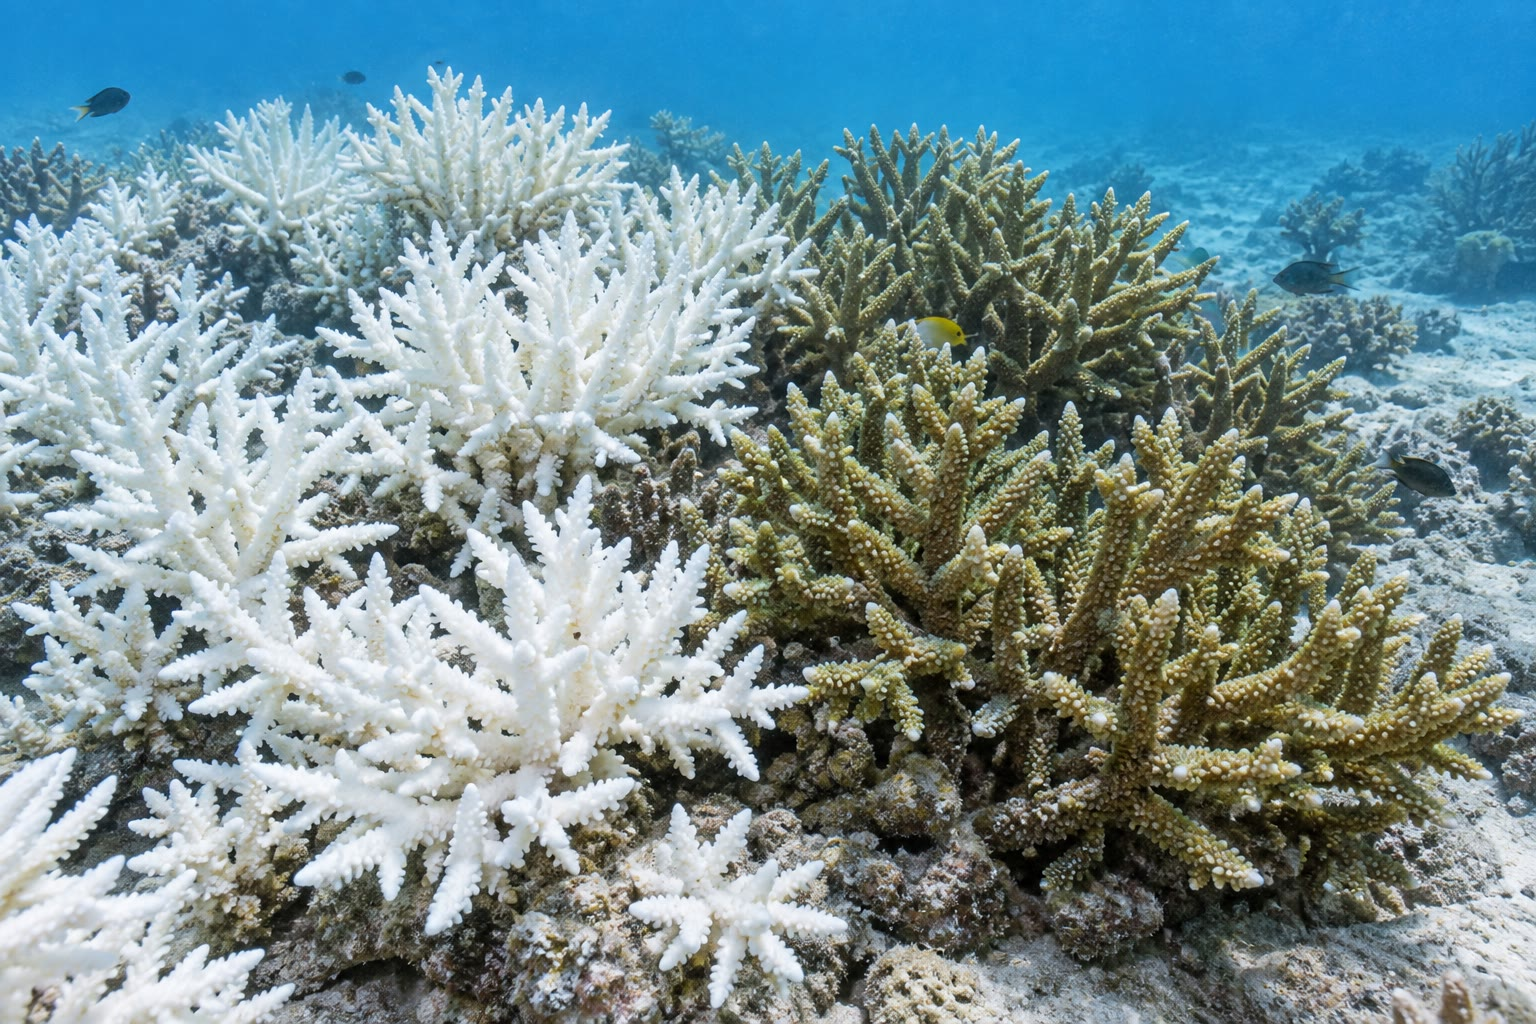
\includegraphics[width=0.56\linewidth]{images/book5/ai/b5-14-coral-bleaching.jpg}

{\small شعبة نصفها مبيضّ: المستعمرات البيضاء طردت طحالبها
بعد أسابيع من ماء شديد الدفء؛ وأما البنية فلا تزال تحمل
طحالبها. والمرجان الأبيض حي جائع، وأمامه أسابيع ليُستعمَر من جديد.}
\end{omfigure}

\begin{omfigure}
\begin{tikzpicture}[every node/.style={font=\scriptsize}, >=stealth]
  % coral cell with alga
  \draw[very thick, omDef, fill=omDef!8] (0,0) ellipse (3.2 and 2.0); \node[above] at (0,2.05) {خلية مرجانية (أديم معدي)};
  \draw[thick, omMeth!70!black, fill=omMeth!30] (-0.4,-0.1) circle (1.05); \node[align=center] at (-0.4,-0.1) {طحلب\\(زوزانثيلة)};
  % exchanges
  \draw[->, thick, omMeth!70!black] (0.5,0.4) -- (1.9,0.9) node[right, align=left] {غليسرول، وسكريات، وأحماض أمينية:\\حتى \qty{90}{\%} من الكربون المثبَّت};
  \draw[<-, thick, omThm] (0.5,-0.5) -- (1.9,-1.0) node[right, align=left] {CO$_2$، وNH$_3$، وفوسفات\\(فضلات الحيوان)};
  \draw[<-, thick, omProp] (-1.3,0.3) -- (-2.6,1.0) node[left, align=right] {ضوء عبر\\النسيج};
  \node[below, align=center] at (1.5,-2.1) {إجهاد: ماء دافئ أسابيع $\to$ تضرر التركيب الضوئي،\\أكسجين فعال $\to$ طرد الطحلب $\to$ ابيضاض};
  % thermometer-like bar on the right
  \begin{scope}[xshift=7.6cm, yshift=-1.6cm]
    \draw[thick] (0,0) rectangle (0.5,3.2);
    \fill[omDef!40] (0,0) rectangle (0.5,2.0); \fill[omProp!60] (0,2.0) rectangle (0.5,2.6); \fill[omThm!60] (0,2.6) rectangle (0.5,3.2);
    \node[right] at (0.6,1.0) {المجال السوي}; \node[right] at (0.6,2.3) {$+\qty{1}{\celsius}$: إجهاد}; \node[right, align=left] at (0.6,2.9) {$+\qty{2}{\celsius}$ أسابيع:\\ابيضاض};
    \node[below, align=center] at (0.25,-0.1) {حرارة البحر\\صيفًا};
  \end{scope}
\end{tikzpicture}

{\small مبادلة المرجان والطحلب: يثبّت الطحلب الكربون
بفضلات الحيوان وبالضوء العابر لنسيجه ويعيد معظمه غذاءً؛
وارتفاع صغير مستمر في الحرارة يكسر الشراكة.}
\end{omfigure}

\section{من شريك إلى عضية}

\begin{proposition}[اختزال الجينوم والطريق إلى العضية]\label{prop:b3:microbiomes:reduction}
\index{اختزال الجينوم}\index{نقل مورّثات تعايشي داخلي}
المتعايش الداخلي الموروث عبر البيضة يعيش في جمهرة من خلايا
قليلة لا تتأشب قط مع خارجها. فالانتخاب عليه ضعيف
(\cref{ch:b3:molecular-evolution}: فالجمهرة الصغيرة تثبّت
بالانجراف طفرات ضارة ضررًا طفيفًا)، والمورّثات التي يوفر
المضيف منتجاتها لا تُفتقد إذا تعطلت، والمورّثة المفقودة لا
تُستعاد أبدًا. فيتقلص الجينوم إذن جيلًا بعد جيل ---
\emph{Buchnera} إلى \qty{640}{kb}، وبعض متعايشات الحشرات
إلى \qty{140}{kb} وبضع مئات من المورّثات، والمتقدرة إلى
\qty{16}{kb} وثلاثة عشر بروتينًا في الإنسان --- وتكتسب نواة
المضيف نسخًا من مورّثات المتعايش \emph{\omterm{prop:b3:microbiomes:reduction}{بنقل مورّثي تعايشي}
داخلي}، وتُستورد منتجاتها راجعةً بمتوالية استهداف. وحين
يصنع المضيف معظم بروتينات المتعايش، ويتحكم بانقسامه، ولا
يقدر على العيش بدونه، يكون المتعايش قد صار عضية. وقد سلكت
المتقدرات والبلاستيدات هذا الطريق قبل ملياري سنة ومليار
سنة (مجلد السنة الأولى)؛ وكروماتوفور \emph{Paulinella}
مسافر ثالث، قطع مئة مليون سنة منه.
\end{proposition}

\begin{remark}[عودة إلى الفرد]\label{rem:b3:microbiomes:individual}
الحيوان أو النبات جماعة في مركزها جينوم، ويتوقف معظم
ذخيرتها الاستقلابية، وكثير من نمائها ومناعتها، على شركاء
لم ترثهم في DNA نفسها. والنتائج العملية حاضرة من الآن:
\omterm{def:b3:microbiomes:symbiosis}{فالميكروبيوم} دواء (زرع البراز)، وهدف للأدوية (الضرر
الجانبي للصادات، والألياف الغذائية وصفةً طبية)، ووسيلة
تشخيص، وسبيل --- عبر المتعايشات المهندَسة والبعوض الحامل
\emph{Wolbachia} --- إلى تغيير بيولوجيا الجمهرات البرية.
وأما النتيجة النظرية فهي أن الانتخاب الطبيعي يعمل على
الشراكات، وأن أقوى الشراكات ما يكون فيها مصير أحد الشريكين
مصير الآخر.
\end{remark}

\section{تمارين}

\begin{exercise}[$\star$]\label{exo:b3:microbiomes:1}
عرّف \omterm{def:b3:microbiomes:symbiosis}{التقايض} \omterm{def:b3:microbiomes:symbiosis}{والمعايشة} والتطفّل، واذكر مثالًا على كل منها
من هذا الفصل. ولماذا يمكن لزوج واحد من الأنواع أن ينتقل
بين الفئات؟
\end{exercise}

\begin{exercise}[$\star$]\label{exo:b3:microbiomes:2}
احسب $H$ و$e^{H}$ و$D$ و$1/D$ لجماعة وفراتها
$0.5$ و$0.3$ و$0.1$ و$0.05$ و$0.05$.
\end{exercise}

\begin{exercise}[$\star$]\label{exo:b3:microbiomes:3}
قابل بين مسح مُضخَّمات 16S وميتاجينوميات البندقية: بماذا
يخبر كل منهما، وما الذي لا يستطيع كل منهما أن يقوله لك؟
\end{exercise}

\begin{exercise}[$\star$]\label{exo:b3:microbiomes:4}
اذكر أربع خدمات يقدمها \omterm{def:b3:microbiomes:gut}{ميكروبيوم الأمعاء} لمضيفه، ومرضًا
واحدًا يتلو اختلاله.
\end{exercise}

\begin{exercise}[$\star\star$]\label{exo:b3:microbiomes:5}
عينة من $N = 20$ قراءة فيها أنواع عند $N_{i} = 10, 6, 3, 1$.
احسب $E[S_{n}]$ عند $n = 5$ من المبرهنة، واحسب \omterm{thm:b3:microbiomes:rarefaction}{تغطية غود}.
\end{exercise}

\begin{exercise}[$\star\star$]\label{exo:b3:microbiomes:6}
يحوي القولون \qty{400}{g} من المحتويات عند $10^{11}$ بكتيريا
في الغرام؛ وتزن البكتيريا الواحدة \qty{1}{pg} وفي جينومها
\num{4000} مورّثة؛ وفي أمعاء الشخص $1000$ نوع. قدّر كتلة
\omterm{def:b3:microbiomes:symbiosis}{الميكروبيوم} وعدد المورّثات المتمايزة التي يحملها، وقارن
بمورّثات الجينوم البشري \num{20000}.
\end{exercise}

\begin{exercise}[$\star\star$]\label{exo:b3:microbiomes:7}
اشرح مفارقة الأكسجين في العقدة، وكيف يحلها \omterm{def:b3:microbiomes:nodule}{الليغهيموغلوبين}
وحاجز الانتشار. ولماذا تكون العقدة وردية، وماذا تعني عقدة
خضراء؟
\end{exercise}

\begin{exercise}[$\star\star$]\label{exo:b3:microbiomes:8}
طافر بقولي يفتقر إلى مكوّن تذبذب الكالسيوم في \omterm{def:b3:microbiomes:mycorrhiza}{سبيل التعايش
المشترك}. تنبأ بقدرته على تكوين العقد وعلى تكوين \omterm{def:b3:microbiomes:mycorrhiza}{الميكوريزا}،
واشرح ما يقوله ذلك عن تطور التعايشين.
\end{exercise}

\begin{exercise}[$\star\star$]\label{exo:b3:microbiomes:9}
صف تجربة العقوبات عند كيرز، وما الذي كان سيُتوقع لو لم
يقدر النبات على تمييز العقد المثبّتة من غير المثبّتة.
\end{exercise}

\begin{exercise}[$\star\star\star$]\label{exo:b3:microbiomes:10}
برهن على أن $E[S_{n}]$ في مبرهنة \omterm{def:b3:microbiomes:diversity}{الترقيق} دالة متزايدة في
$n$ وتبلغ $S$ عند $n = N$، وبيّن أن نوعًا عند
$N_{i} \ll N$ و$n \ll N$ احتمال رؤيته يقارب
$1 - (1 - n/N)^{N_{i}}$.
\end{exercise}

\begin{exercise}[$\star\star\star$]\label{exo:b3:microbiomes:11}
\emph{Wolbachia} لا تنتقل إلا عبر البيوض. اشرح لماذا يحابي
الانتخاب عليها المضائف الإناث، وصف عدم التوافق
السيتوبلازمي، وبيّن لماذا يتيح لسلالة مصابة أن تنتشر ولو
حمل الخمج كلفة صغيرة.
\end{exercise}

\begin{exercise}[$\star\star\star$]\label{exo:b3:microbiomes:12}
استنادًا إلى \cref{prop:b3:microbiomes:reduction}، اشرح لماذا
تتقلص جينومات المتعايشات الداخلية المنقولة عموديًا ولا
تتقلص جينومات أقاربها الحرة، وأي المورّثات تُفقد أولًا
وأيها آخرًا، وما الذي يعكس هذا الاتجاه.
\end{exercise}

\section{مسألة: تعداد أمعاء}

\begin{problem}[{مسألة نهاية الأسبوع --- ميكروبيوم أمعاء يُعدّ
بالخلايا والمورّثات والسعرات، ويُقاس تنوعه ويُرقَّق،
وتُوازَن ميزانية نتروجين بقولية في مقابل سكرها، ويُحسب
كربون شعبة مرجانية، وتُختم بالسعرات التي يكسبها ميكروبيوم،
وتغطية عينة تسلسل، والسكر الذي يدفعه حقل فول ثمنًا
لنتروجينه}]
\label{pb:b3:microbiomes:1}
المعطيات: محتويات القولون \qty{400}{g} عند $10^{11}$ بكتيريا
في الغرام، وكتلة الخلية \qty{1}{pg}؛ و$1000$ نوع، في كل
منها \num{4000} مورّثة، و\qty{30}{\%} من المورّثات مشتركة
بين أي نوعين. والحمية: \qty{30}{g} من الألياف يوميًا،
تُخمَّر إلى أحماض دهنية قصيرة السلسلة بمعدل \qty{10}{mmol}
للغرام، قيمة كل منها \qty{0.9}{kJ}؛ والحمية \qty{9000}{kJ}.
وعينة تسلسل: $N = 2000$ قراءة، و$S = 180$ نوعًا، و$f_{1} = 60$
نوعًا مفردًا؛ ووفرات الأنواع الثلاثة الأولى $0.30$ و$0.20$
و$0.10$، والباقي موزع بالتساوي. ومحصول فول يثبّت
\qty{150}{kg} من N في الهكتار في الموسم ويدفع \qty{8}{g} من
السكر لكل غرام من N مثبَّت؛ وتركيبه الضوئي يعطي \qty{12}{t}
من السكر في الهكتار في الموسم. \omterm{def:b3:microbiomes:nodule}{والنتروجيناز}: $16$ ATP لكل
N$_{2}$. ومرجان: $10^{6}$ طحلب في cm$^{2}$، يثبّت كل منها
\qty{20}{pg} من الكربون يوميًا، ويمر \qty{90}{\%} منه إلى
المضيف؛ ونسيج المرجان يتنفس \qty{15}{\micro g} من الكربون
في cm$^{2}$ يوميًا.

\medskip
\noindent\textbf{الجزء الأول --- الخلايا والمورّثات.}
\begin{enumerate}
  \item كم بكتيريا في القولون، وكم تزن؟
  \item كم يعادل ذلك من جينومات بكتيرية من DNA، وكيف يقارَن
        المجموع مع DNA الموجود في $3\times 10^{13}$ خلية
        بشرية (\qty{6.4}{pg} لكل منها)؟
  \item قدّر عدد المورّثات البكتيرية المتمايزة في الأمعاء،
        مع مراعاة التداخل \qty{30}{\%} (عُدّ \qty{70}{\%} غير
        المشتركة من كل نوع مضافًا إليها مجموعة مشتركة
        واحدة). وقارن مع \num{20000}.
  \item كم ميلي مول من الأحماض الدهنية القصيرة السلسلة
        تعطي الألياف يوميًا، وكم كيلوجول، وأي نسبة من
        الحمية؟
  \item يحتاج الفأر الخالي من الجراثيم إلى \qty{30}{\%} طعام
        أكثر. فهل إسهام الأحماض الدهنية في السؤال 4 يكفي
        لتفسير ذلك؟ وما الذي قد يفسره أيضًا؟
  \item تنقسم البكتيريا في القولون مرة في اليوم تقريبًا،
        وتُطرح المحتويات بالمعدل نفسه. فأي حالة مستقرة
        يقتضي ذلك، وماذا يحدث للجماعة حين يقتل شوط من
        الصادات \qty{99.9}{\%} من الخلايا؟
\end{enumerate}

\medskip
\noindent\textbf{الجزء الثاني --- التنوع.}
\begin{enumerate}[resume]
  \item احسب الوفرة النسبية لكل نوع من الأنواع الثانوية
        $177$، ثم \omterm{def:b3:microbiomes:diversity}{دليل شانون} $H$ و$e^{H}$.
  \item احسب \omterm{def:b3:microbiomes:diversity}{دليل سيمبسون} $D$ و$1/D$. ولماذا يكون $1/D$
        أصغر من $e^{H}$؟
  \item ما \omterm{thm:b3:microbiomes:rarefaction}{تغطية غود} للعينة؛ وكم قراءة في الألف تنتمي إلى
        أنواع لم تُرَ؟
  \item عينة ثانية من \num{10000} قراءة من الأمعاء نفسها
        تعطي $260$ نوعًا. اشرح، مستعملًا مبرهنة \omterm{def:b3:microbiomes:diversity}{الترقيق}،
        لماذا ليس في ذلك تناقض، وماذا يجب أن يُفعل قبل
        مقارنة العينتين.
  \item في المبرهنة، ما احتمال أن يظهر نوع عند
        $N_{i} = 1$ في عينة جزئية من $n = 1000$ من $N =
        2000$؟ وعند $N_{i} = 5$؟
  \item بعد الصادات تُظهر الأمعاء نفسها $60$ نوعًا،
        و$H = 2.0$، ونوعًا واحدًا عند وفرة $0.5$. احسب
        $e^{H}$ و$D$ وصف الجماعة بالكلام.
\end{enumerate}

\medskip
\noindent\textbf{الجزء الثالث --- حساب العقدة.}
\begin{enumerate}[resume]
  \item كم سكرًا يدفع المحصول في الهكتار مقابل \qty{150}{kg}
        من N، وأي نسبة من تركيبه الضوئي ذلك؟
  \item كم مولًا من N$_{2}$ تعادل \qty{150}{kg} من N، وكم
        مولًا من ATP ينفق \omterm{def:b3:microbiomes:nodule}{النتروجيناز} عليها؟
  \item عند $30$ ATP لكل غلوكوز يُتنفس، كم كيلوغرامًا من
        الغلوكوز يمثل ذلك؟ وقارن بالسكر المدفوع؛ وفيم
        الباقي؟
  \item يكلف النشادر الصناعي نحو \qty{35}{MJ} لكل كيلوغرام
        من N. مستعملًا \qty{16}{kJ} للغرام من السكر، قارن
        كلفة طاقة نتروجين المحصول بكلفة المصنع.
  \item يدخل ريزوبيوم غير مثبّت عقدةً. فإذا عاقبه النبات
        بتنصيف أكسجينه، وهبط تكاثره إلى النصف، فأي نسبة من
        \omterm{def:b3:microbiomes:nodule}{ريزوبيا} الموسم التالي غشّاشة إذا بدأت عند
        \qty{10}{\%} وتكاثرت المثبّتات تكاثرًا سويًا؟
        (جولة واحدة.)
  \item من دون عقوبات، تتكاثر الغشّاشات التي توفر كلفة
        التثبيت \qty{20}{\%} أكثر. فعلى عشرة مواسم، أي نسبة
        تكون غشّاشة، من البداية نفسها؟ وماذا تبيّن المقارنة؟
\end{enumerate}

\medskip
\noindent\textbf{الجزء الرابع --- حساب الشعبة.}
\begin{enumerate}[resume]
  \item كم كربونًا تثبّت طحالب سنتيمتر مربع واحد يوميًا،
        وكم يبلغ المرجان منه؟
  \item قارن بتنفس المرجان. ما الفائض، وفيم يُستعمل؟
  \item بعد الابيضاض تختفي \qty{95}{\%} من الطحالب. أعد حساب
        الكربون المورَّد. وكم يدوم المرجان على مخزون قدره
        \qty{300}{\micro g} من الكربون في cm$^{2}$؟
  \item كثيرًا ما يُقاس الإجهاد بأسابيع-درجات التسخين: أي
        مجموع الفائض الأسبوعي فوق العظمى الصيفية على مدى
        الموسم. فثمانية أسابيع عند $+\qty{1}{\celsius}$ أو
        أربعة عند $+\qty{2}{\celsius}$ كلاهما يعطي $8$؛
        ويبدأ الابيضاض قرب $4$. فأي المسارين أسوأ، ولماذا
        قد يصلح المقياس مع ذلك؟
  \item يمكن للمرجان أن يؤوي أنواعًا طحلبية عدة بحدود
        حرارية مختلفة. اقترح كيف يمكن لشعبة أن تتأقلم، وما
        الذي يحد من ذلك.
  \item شعبة من \qty{1}{km^2} من سطح المرجان الحي: كم
        كربونًا تثبّت طحالبها يوميًا وسنويًا، بالأطنان؟
  \item لخّص: نسبة الحمية التي يوفرها \omterm{def:b3:microbiomes:symbiosis}{الميكروبيوم}
        (السؤال~4)، وتغطية عينة التسلسل (السؤال~9)، ونسبة
        التركيب الضوئي التي يدفعها محصول الفول مقابل
        نتروجينه (السؤال~13).
\end{enumerate}
\end{problem}
